\documentclass{article}
\usepackage[utf8]{inputenc}
\usepackage{titling}
\usepackage{graphicx}
\usepackage{xcolor}
\usepackage[colorlinks=true,linkcolor=darkgray, urlcolor =gray]{hyperref}
\usepackage[spanish]{babel}
\DeclareUnicodeCharacter{301}{~}
\usepackage{url}
\DeclareUnicodeCharacter{202F}{\,}


\title{Evaluación tecnológica de soluciones de gestión comercial para PYMES}
\author{Álvaro Fernández Palma\\ Alina Altynguzhina\\ Iman Hasnaouia Meskini\\ Cristina Díaz García}
\date{October 2018}

\renewcommand\maketitlehooka{\null\mbox{}\vfill}
\renewcommand\maketitlehookd{\vfill\null}


\begin{document}

\addcontentsline{toc}{section}{Índice general}

\begin{titlingpage}
\maketitle

\begin{center}

\includegraphics[scale=0.5]{imagenes/gestioncomercial.jpg} 
\end{center}

\end{titlingpage}

\newpage

\tableofcontents

\newpage

\section{Plan de Trabajo}

\subsection{Tareas}

Describir y evaluar un total de seis softwares de solución de gestión comercial para empresas de los siguientes tipos y asignados a las siguientes personas: 

\textbf{Software de tipo Propietario:} Alina (Gespymes) e Iman (Sage 50 Cloud). 

\textbf{Software de tipo Libre:} Cristina (Odoo). 

\textbf{Software de tipo SaaS:} Alina (ZFactura) y Álvaro (Galdon). 

\textbf{Software de tipo Movilidad:} Iman (Repcamp). 

\textbf{Presentación:} Cristina 

 

\subsection{Planificación temporal}

Hasta el día 27 de octubre hay que buscar información sobre el tipo de software que se le ha sido asignado. 
Hasta el día 1 de noviembre, analizar software y valorarlo. 
Hasta el día 4 de noviembre, realizar informe.


\section{Modelo de Calificación}

\subsection{Criterios funcionales}

\begin{itemize}
	\item \textbf{TPV (point of sale):} Dispositivo que usan los establecimientos comerciales para realizar gestiones de venta. Las funciones que incluye son: pagos con tarjeta, devolución de pagos con tarjeta, control de inventario, creación de facturas, etc. 
	\item \textbf{Gestión del catálogo y precios:} Herramienta que permite visualizar los productos, la cantidad de productos de la que se dispone, su precio (con y sin impuestos) y otros datos según convenio. 
	\item \textbf{Gestión de devoluciones y cancelaciones:} Herramienta que permite visualizar la devolución de productos o la cancelación de la compra de un producto. 
	\item \textbf{Facturación:} Generación de facturas, documento en el cual se puede ver la información de una compra, venta y/o devolución. 
	\item \textbf{Reserva de productos:} Posibilidad de reservar o no productos antes de su compra, además, de manera cómoda y eficiente.
	\item \textbf{Generación de informes:} Generación automática de informes de compras, ventas, inventario, facturas, etc de manera rápida y cómoda.
	\item \textbf{Soporte para métodos de pago:} Posibilidad de pagar con distintos métodos de pago como efectivo, tarjeta, NFC, entre otros.
\end{itemize}


\subsection{Criterios no funcionales}

\begin{itemize}
	\item \textbf{Coste:} Coste mensual/anual/único que se debe abonar para disponer del software.
	\item \textbf{Evolución:} Mejoras que ha tenido el software con el tiempo. 
	\item \textbf{Posibilidad de personalización:} La posibilidad de poder personalizar tanto de manera estética como funcional. 
	\item \textbf{Casos de éxito:} Casos reales en los cuales utilizando el software, se ha llegado a un proyecto exitoso.  
\end{itemize}

\subsection{Descripción de la escala de ponderación}

Hemos utilizado una escala de ponderación del 1 al 4, siendo el 1 el valor que atribuye menos importancia al criterio y 4 el valor que atribuye mayor valor al criterio, afectando así a la influencia del criterio en la calificación. 

Hemos utilizado esta escala de ponderación porque al tener pocos criterios, con pocos valores es más fácil y sencillo asignar un valor de ponderación a cada criterio. 

\section{Descripción y estudio de los softwares elegidos}

\subsection{Softwares Propietarios}

\subsubsection{Sage 50 Cloud}
	
	Sage 50 Cloud es un software propietario (ya que requiere de pago mensual o anual) de gestión comercial que permite gestionar las áreas básicas de un negocio. 
	
\begin{flushleft}
	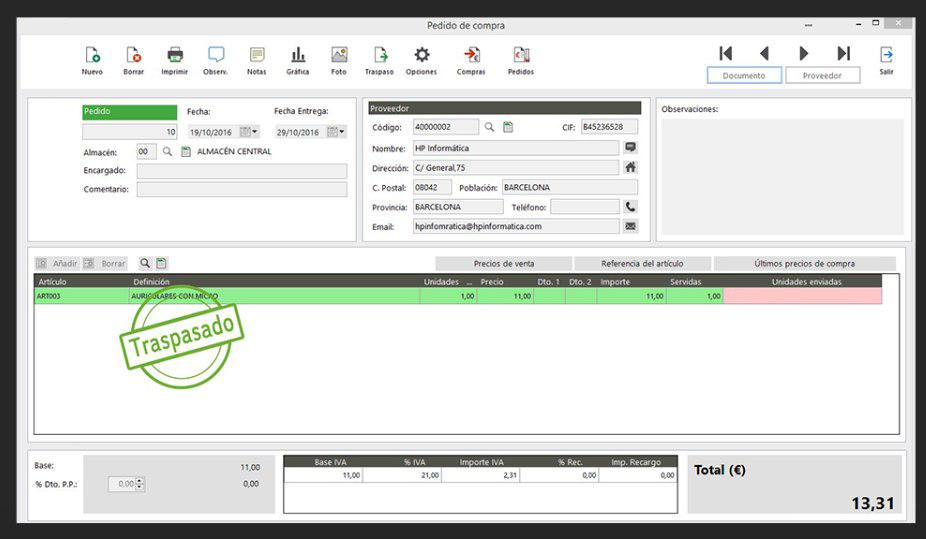
\includegraphics[scale=0.5]{imagenes/sage50.jpg} 
\end{flushleft}	

\begin{flushleft}
	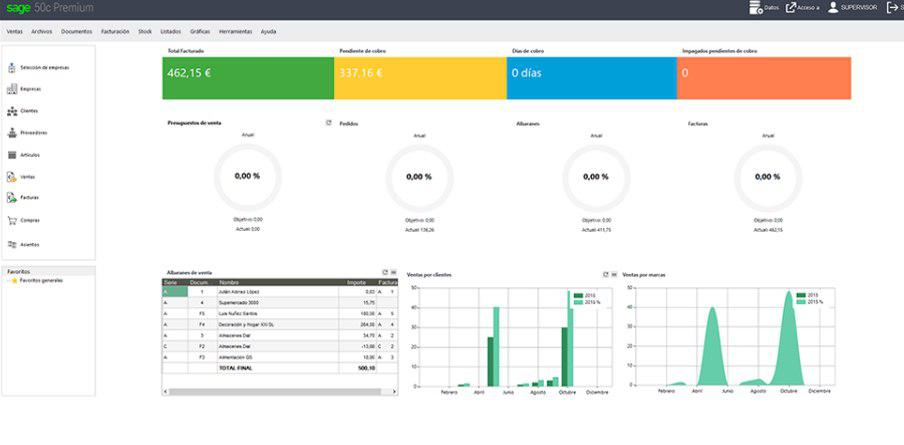
\includegraphics[scale=0.75]{imagenes/sage50_2.jpg} 
\end{flushleft}

\paragraph{Criterios funcionales:}

\begin{itemize}

	\item \textbf{TPV (point of sale):} Funcionalidad completa: punto de venta, compras, ventas, almacén, stocks, etc. 
	\item \textbf{Gestión del catálogo y precios:} Personalizable.
	\item \textbf{Gestión de devoluciones y cancelaciones:} Personalizable.
	\item \textbf{Facturación:} Incluido en la generación de informes, documento multiplataforma, seguro y personalizable. 
	\item \textbf{Reserva de productos:} Personalizable.
	\item \textbf{Generación de informes:} Generación de documentos personalizada y segura.
	\item \textbf{Soporte para métodos de pago:} El Punto de Venta proporciona un soporte para múltiples métodos de pago.

\end{itemize}

\paragraph{Criterios no funcionales:}

\begin{itemize}

	\item \textbf{Coste:} Desde 45,36 euros al mes o 499 euros al año. 
	\item \textbf{Evolución:} Al incluir herramientas necesarias siempre, la evolución es positiva
	\item \textbf{Posibilidad de personalización:} Totalmente personalizable.
	\item \textbf{Casos de éxito:} Handling Truck Services.

\end{itemize}

\paragraph{Evaluación de Sage 50 Cloud}

\begin{flushleft}
	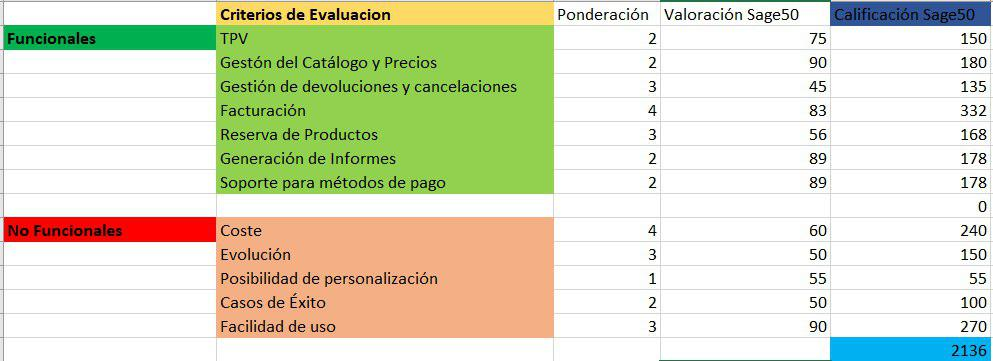
\includegraphics[scale=0.6]{imagenes/Sage50.jpg} 
\end{flushleft}

\subsubsection{ZFactura}

	ZFactura es uno de programas de facturación especializado para pymes, autónomos y profesionales independientes que permite configurar múltiples modelos de facturas, plantillas de presupuestos mediante un potente editor de informes incluído. 

Con el programa de gestión para pymes ZFactura puede gestionar sus archivos de datos como: 

\begin{itemize}
	\item Productos y servicios.
	\item Clientes.
	\item Proveedores.
	\item Gastos – Facturas de compra.
	\item Presupuestos de venta.
	\item Facturas proforma.
	\item Ingresos – Facturas de venta.
	\item Facturas rectificativas.
	\item Facturas periódicas.
	\item Factura electrónica.
	\item Agenda, avisos y alarmas.
\end{itemize}

\begin{flushleft}
	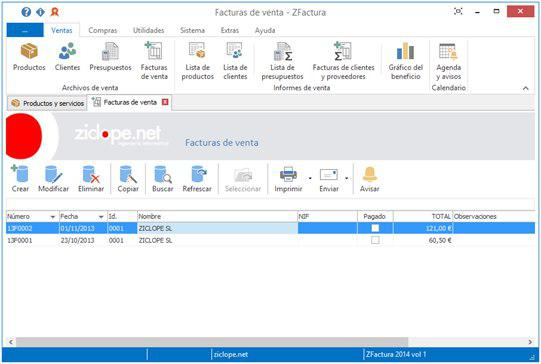
\includegraphics[scale=0.6]{imagenes/ZFactura.jpg} 
\end{flushleft}

\paragraph{Criterios funcionales:}

\begin{itemize}

	\item \textbf{TPV (point of sale):} Las funciones que incluye son: pagos con tarjeta, control de inventario, creación de facturas, etc. 
	\item \textbf{Gestión del catálogo y precios:} Personalizable.
	\item \textbf{Gestión de devoluciones y cancelaciones:} No encontrado.
	\item \textbf{Facturación:} Facturas proforma, de venta, rectificativas, periódicas, electrónicas.  
	\item \textbf{Reserva de productos:} Personalizable.
	\item \textbf{Generación de informes:} Dispone de un gestor de informes que le permite diseñar sus propios modelos de facturas, plantillas de presupuestos, incluyendo datos adicionales como logotipos, direcciones alternativas. ZFactura viene acompañado de diversos modelos de facturas y otros informes predefinidos.
	\item \textbf{Soporte para métodos de pago:} Personalizable, además en versión 2017 se integró la posibilidad de pagar con PayPal al enviar un presupuesto o factura.  

\end{itemize}

\paragraph{Criterios no funcionales:}

\begin{itemize}

	\item \textbf{Coste:} Estándar (99eu), profesional (199eu) y personalizado (399eu). 
	\item \textbf{Evolución:} En versión 2019, han incluido gestor de envío de newsletters.  
En 2017, han añadido visor de mapas de google en clientes y proveedores que permite con un clic ver su ubicación. En 2012, módulo de exportación de datos a Excel, HTML y CSV. Y muchas novedades más cada año.  
	\item \textbf{Posibilidad de personalización:} Se puede personalizarlo con el plan personalizado.  
	\item \textbf{Casos de éxito:} Los programas están orientados a autónomos y pequeñas empresas, pero se pueden destacar algunas empresas e instituciones muy relevantes que han confiado en este software debido a su calidad y eficiencia: 
	\begin{itemize}
		\item Bankia 
		\item Junta de Andalucía
		\item La Razón
		\item Universidad de Barcelona 
	\end{itemize}

\end{itemize}

\paragraph{Evaluación de ZFactura}

\begin{flushleft}
	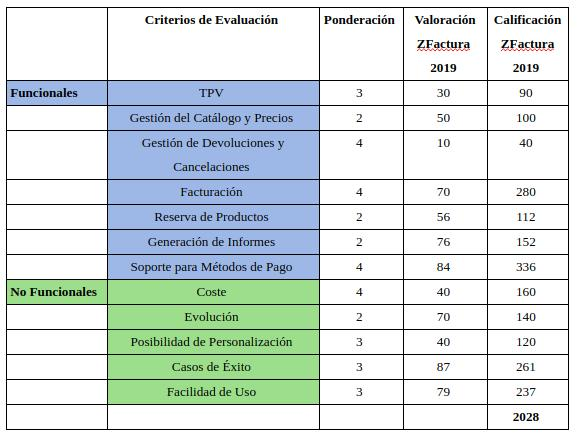
\includegraphics[scale=0.6]{imagenes/EvaluacionZFactura.jpg} 
\end{flushleft}

\subsection{Softwares Libres}

\subsubsection{Odoo}

Odoo es un conjunto de aplicaciones empresariales de código abierto que cubren todas las necesidades de su empresa: CRM, comercio electrónico, contabilidad, inventario, puntos de venta, gestión de proyectos, etc.

\paragraph{Criterios funcionales:}

\begin{itemize}

	\item \textbf{TPV (point of sale):} Tiene una app con versión de restaurante y de comercio, que incluye, entre otras funciones, cuenta dividida y escaneo de códigos, respectivamente. En ambos se pueden tener varias compras simultáneas. Se puede usar tanto online como offline. 
	\item \textbf{Gestión del catálogo y precios:} Personalizable.
	\item \textbf{Gestión de devoluciones y cancelaciones:} Personalizable.
	\item \textbf{Facturación:} Personalizable.
	\item \textbf{Reserva de productos:} Personalizable.
	\item \textbf{Generación de informes:} Generación de documentos personalizada.
	\item \textbf{Soporte para métodos de pago:} Métodos de pago en efectivo, cheques y tarjeta de crédito están disponibles. También se pueden agregar nuevos tipos de métodos de pago. Un solo pedido se puede pagar como un pago dividido entre varias partes, así como con métodos de pago separados.

\end{itemize}

\paragraph{Criterios no funcionales:}

\begin{itemize}

	\item \textbf{Coste:} Para una única aplicación (puede que para el buen funcionamiento de ésta hagan falta otras, en cuyo caso se señalan automáticamente y cuenta como solo una), su precio es 0 euros para cualquier número de usuarios. Si se necesitara más de una aplicación, usualmente cuesta 120 euros anuales o 15 mensuales por usuario para usarlo en la nube, más el precio de éstas, que es en su mayoría 6 o 12 euros al mes, habiendo también algunas de 18, 24 y 36 euros. Si se quisieran comprar más de una aplicación, se cobrarían todas ellas, ninguna sería gratuita.
	\item \textbf{Evolución:} Al incluir herramientas necesarias siempre, la evolución es positiva
	\item \textbf{Posibilidad de personalización:} Totalmente personalizable.
	\item \textbf{Casos de éxito:} Omnia Solutions, entre otros. Tienen un apartado de testimonios en su web en la que empresas que usan sus herramientas cuentan la experiencia que supone hacerlo.

\end{itemize}

\paragraph{Evaluación de Odoo}

\begin{flushleft}
	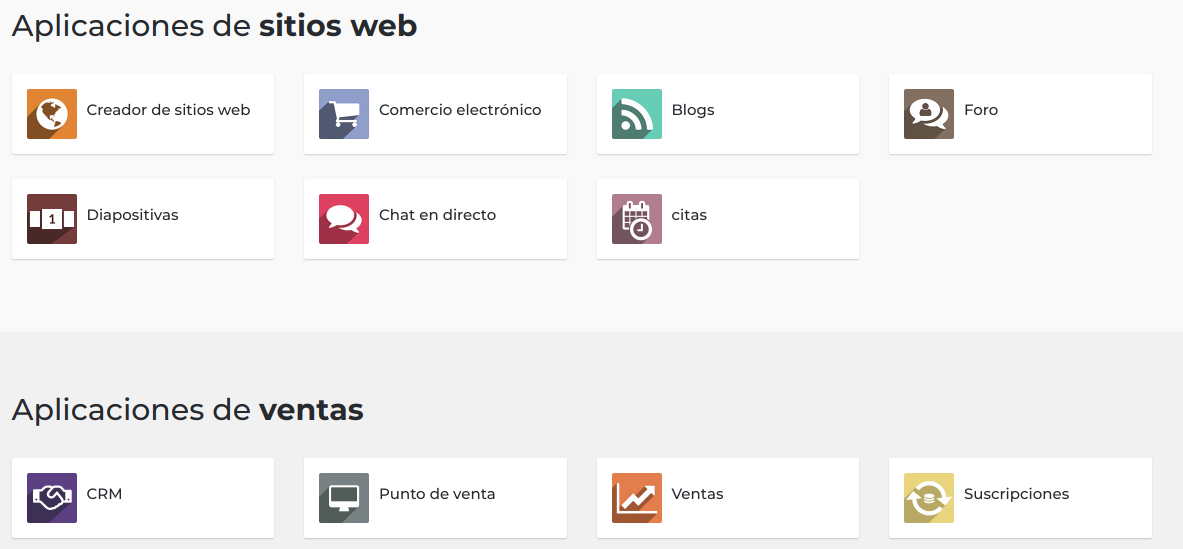
\includegraphics[scale=0.25]{imagenes/Odoo1.png} 
	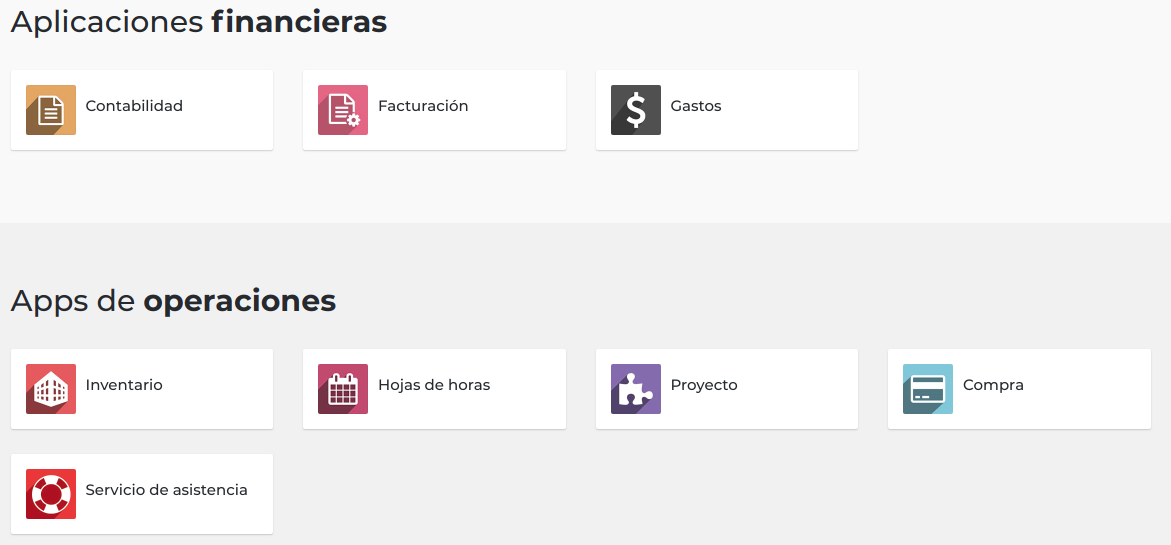
\includegraphics[scale=0.25]{imagenes/Odoo2.png}
	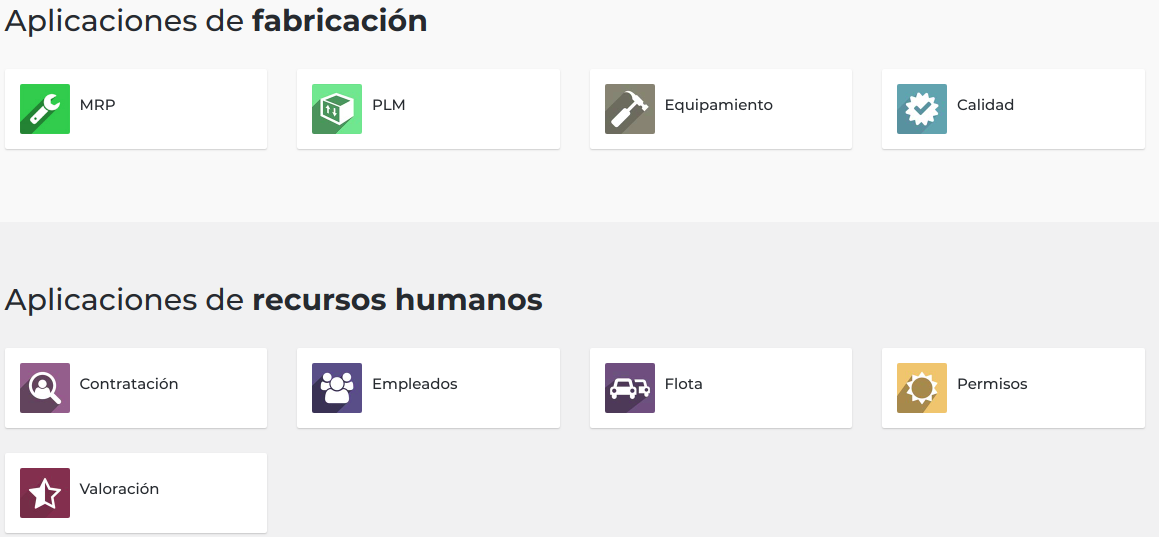
\includegraphics[scale=0.25]{imagenes/Odoo3.png}
	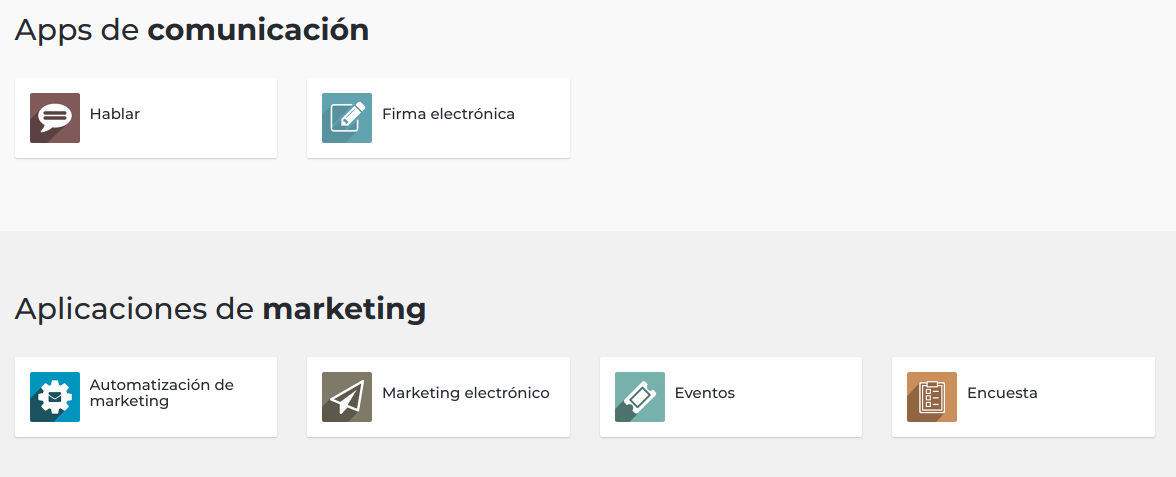
\includegraphics[scale=0.25]{imagenes/Odoo4.png}
	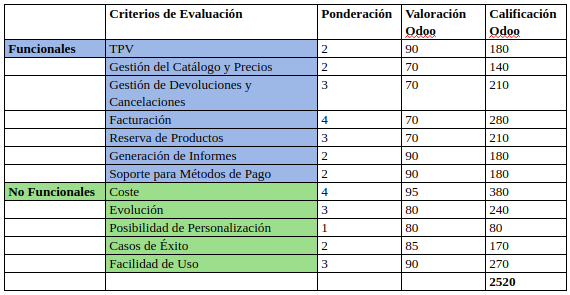
\includegraphics[scale=0.6]{imagenes/EvOdoo.png}
\end{flushleft}

\subsection{Softwares SaaS}

\subsubsection{GesPymes}

GesPymes es un programa propietario de gestión comercial de tipo SaaS.  Integra los apartados de Facturación, Contabilidad online, Cartera de Clientes, Proveedores, Control de Costes, elaboración de Presupuestos, registro de productos, gestionar la parcela comercial, diseño de balances y un largo etcétera. Toda la información está en la nube.

\begin{flushleft}
	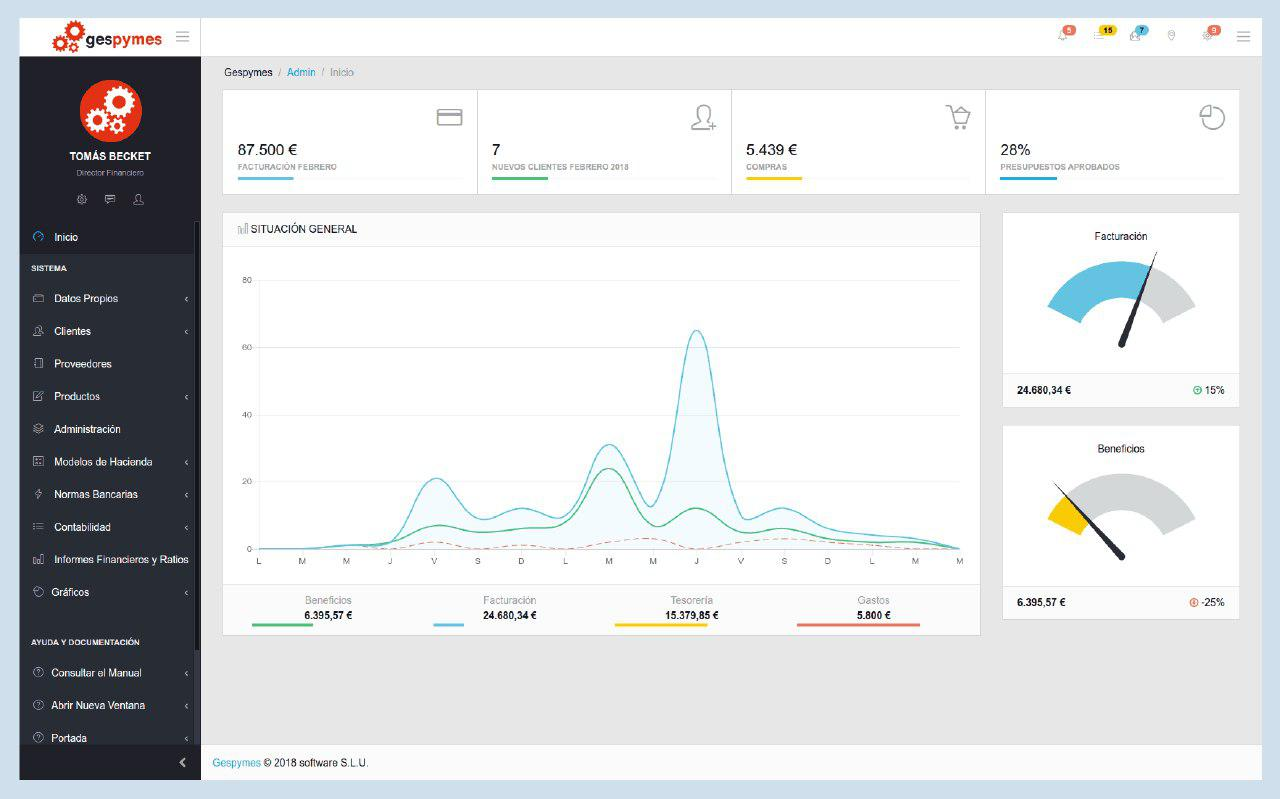
\includegraphics[scale=0.25]{imagenes/Gespymes1.jpg} 
\end{flushleft}

\paragraph{Criterios funcionales:}

\begin{itemize}

	\item \textbf{TPV (point of sale):} Al ser un software tipo SaaS todo se hace en la nube. Personalizable.
	\begin{flushleft}
		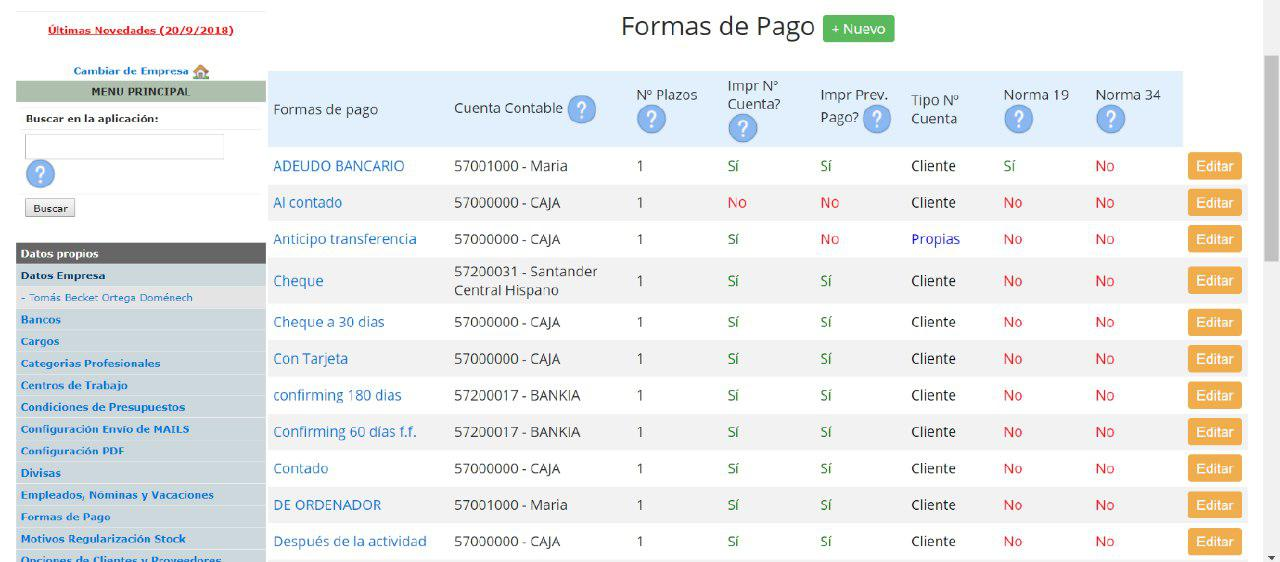
\includegraphics[scale=0.8]{imagenes/Gespymes2.jpg} 
	\end{flushleft}
	\item \textbf{Gestión del catálogo y precios:} Personalizable.
	\item \textbf{Gestión de devoluciones y cancelaciones:} Personalizable.
	\begin{flushleft}
		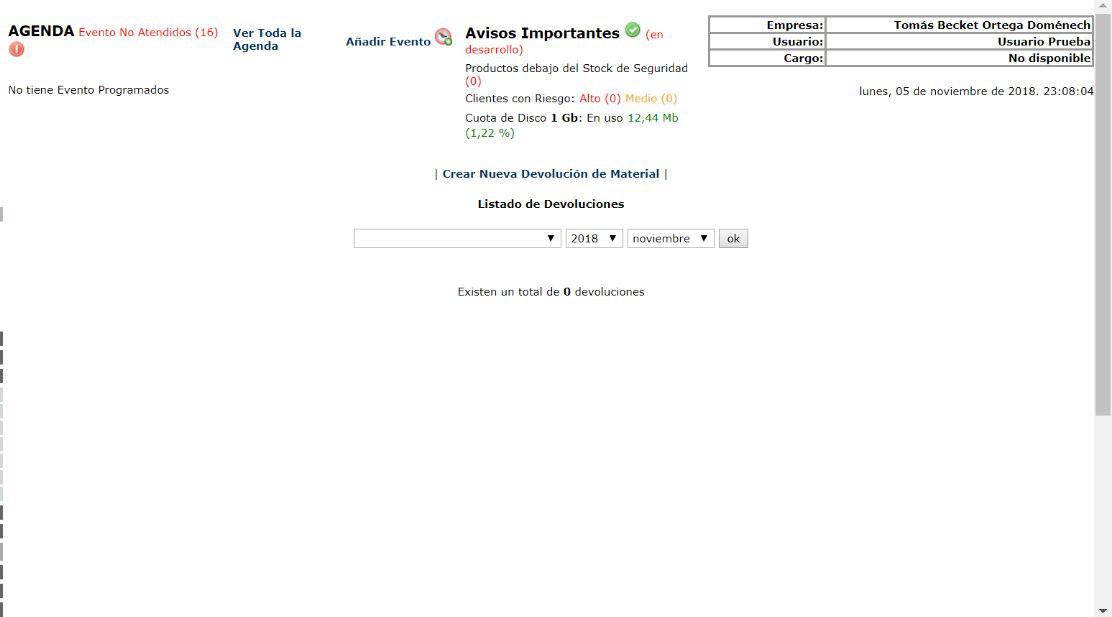
\includegraphics[scale=0.8]{imagenes/gespymes3.jpg} 
	\end{flushleft}
	\item \textbf{Facturación:} aquí podemos ver la facturación para el cliente. Con cambios de divisa, calculando IVA, IRPF, descuentos, retención de garantía. Tiene muchas subdivisiones por proyectos, clientes, por series de facturación, etc.
	\begin{flushleft}
		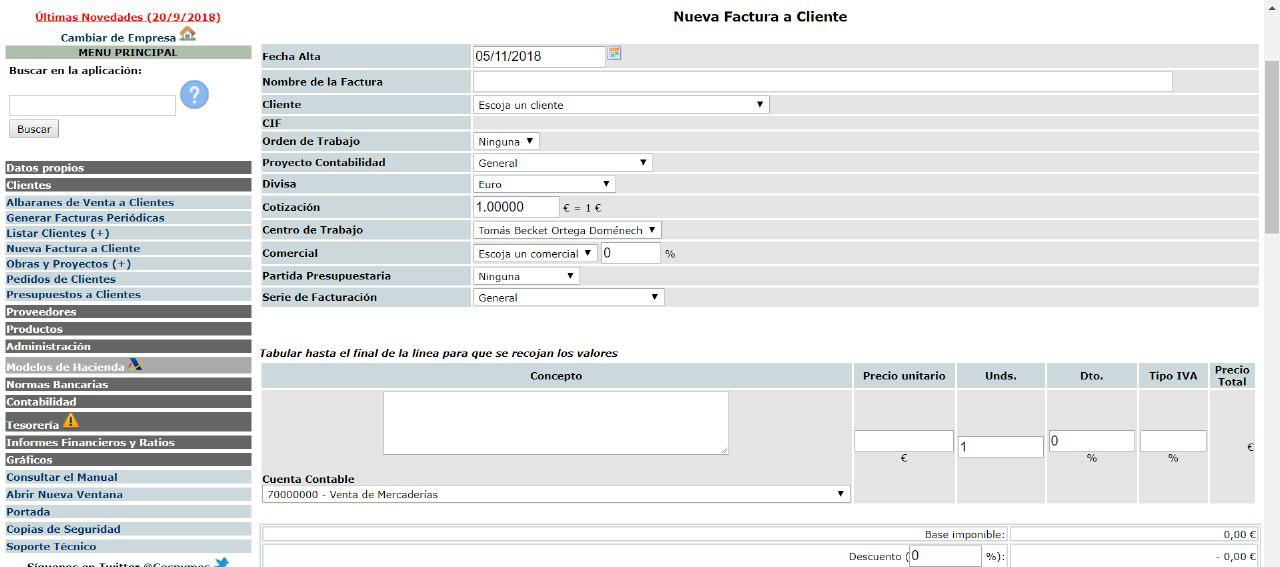
\includegraphics[scale=0.4]{imagenes/gespymes.jpg} 
	\end{flushleft}  
	\item \textbf{Reserva de productos:} Personalizable.
	\item \textbf{Generación de informes:} Generación de informes de compras, ventas, inventario, facturas, etc de manera rápida y cómoda si así lo desea el cliente (hay una opción). Informes por trimestres y por proyectos.
	\begin{flushleft}
		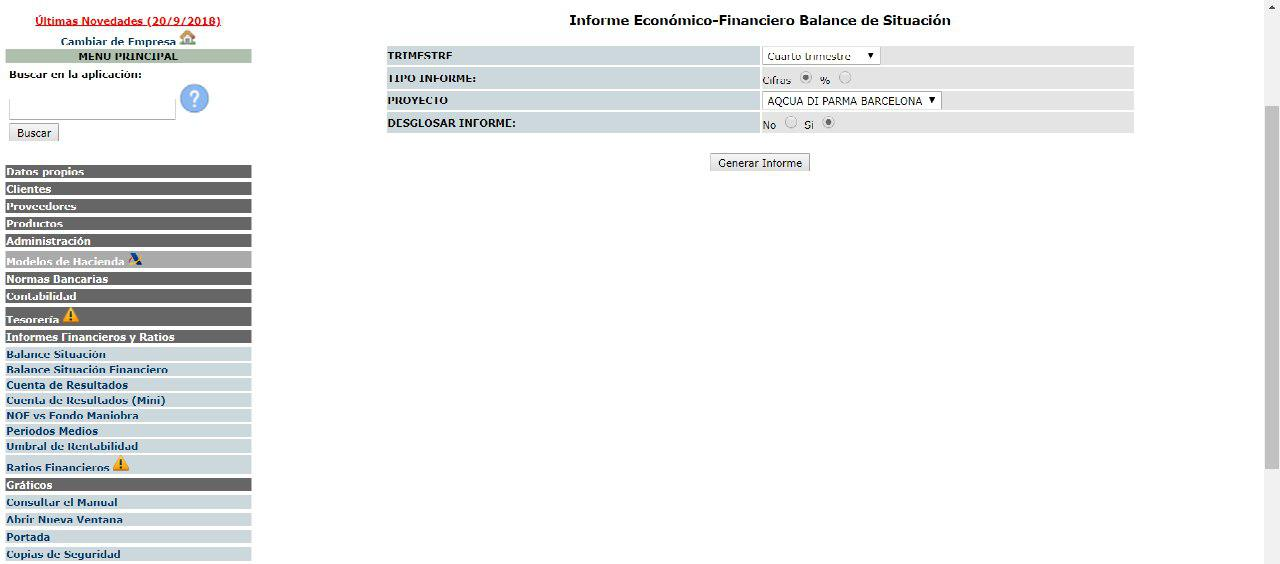
\includegraphics[scale=0.4]{imagenes/gespymes2.jpg} 
	\end{flushleft}  
	\item \textbf{Soporte para métodos de pago:} Personalizable.

\end{itemize}

\paragraph{Criterios no funcionales:}

\begin{itemize}

	\item \textbf{Coste:} El pago es mensual. Plan básico: 9,95. Plan pymes: 29,95. Plan profesional: 39,95. Y la forma de pago es mediante el giro bancario. Aplicación, se cobrarían todas ellas, ninguna sería gratuita.
	\item \textbf{Evolución:} llevan trabajando desde 2006, pero no tenemos ninguna información sobre los cambios realizados, solo a partir de 2015. Y parece que actualizan su software una vez al año. Desde agosto de 2015 han tenido estas actualizaciones:  

\begin{itemize}
	\item Asignar cuentas contables a las formas de pago. 
	\item Listar asientos contables descuadrados 
	\item N.º máximo de días de pago/ cobro de un cliente / proveedor 
	\item Facturas periódicas a clientes  
\end{itemize}
  
	\item \textbf{Posibilidad de personalización:} El programa es configurable, sin embargo, no es posible cambiarlo de forma estética.  
	\item \textbf{Casos de éxito:} No aparece nada en su página web, pero en otras figuran opiniones favorables. Incluso aparece en una lista “20 minutos” en el tercer puesto. También muchos blogs recomiendan el software.  

\end{itemize}

\paragraph{Evaluación de GesPymes}

\begin{flushleft}
	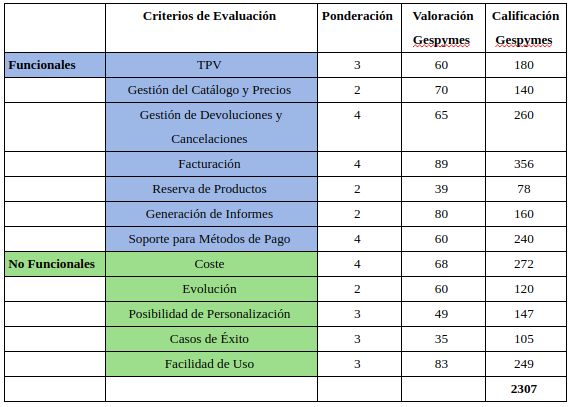
\includegraphics[scale=0.6]{imagenes/GespymesEv.png} 
\end{flushleft}

\subsubsection{Galdon}

\paragraph{Criterios funcionales:}

\begin{itemize}

	\item \textbf{TPV (point of sale):} Únicamente funcionan por contacto vía teléfono o correo, ya que todo el trabajo que realizan es personalizado, los precios deberán de ajustarse en base a las necesidades y requerimientos de cada cliente.  
	\item \textbf{Gestión del catálogo y precios:}  Totalmente personalizado, al gusto del cliente.
	\item \textbf{Gestión de devoluciones y cancelaciones:}  Totalmente personalizado, al gusto del cliente.
	\item \textbf{Facturación:}  Totalmente personalizado, al gusto del cliente . 
	\item \textbf{Reserva de productos:} Totalmente personalizado, al gusto del cliente.
	\item \textbf{Generación de informes:}  Totalmente personalizado, al gusto del cliente .
	\item \textbf{Soporte para métodos de pago:}  Totalmente personalizado, al gusto del cliente.

\end{itemize}

\paragraph{Criterios no funcionales:}

\begin{itemize}

	\item \textbf{Coste:} Indefinido, debido a que tiene multitud de variaciones ya que a cada cliente se le realiza un tipo de trato y se le da un producto prácticamente exclusivo y único para sus necesidades, teniendo pues que contactar personalmente con la empresa y solicitar presupuesto para cada uno de los casos específicos. 
	\item \textbf{Evolución:} Ofrece todo tipo de softwares, todos tipo SaaS pero específicos para cada tipo de necesidad, desde automatizar preventas o automatizarlas desde dispositivos móviles, tablets, etc. Hasta plataformas multiusuario sin duplicidad de información para realizar actualizaciones y modificaciones de todo tipo simultáneamente. Dentro del servicio SaaS que ofertan únicamente hablan de un servicio por tiempo a cuota mensual y no por número de clientes, pudiendo así utilizar el software donde queramos, cuanto queramos y quiénes queramos en el límite de tiempo establecido, aunque nuevamente sin dar datos claros del coste del software.
	\item \textbf{Posibilidad de personalización:} Galdon desde sus inicios, se ha dedicado al desarrollo de gestión a medida y a la necesidad de cada uno de sus clientes, lo cual el grado de personalización es muy alto, tanto como los propios diseñadores y programadores de Galdon quieran y se lo exijan sus clientes. 
	\item \textbf{Casos de éxito:} Vienen en el footer de la página de una de sus secciones, en forma de Slider, de empresas que han trabajado con ellos:
	
\begin{flushleft}
	
\includegraphics[scale=0.4]{imagenes/CapturasoftwareSaaS1o.png} 
	
\includegraphics[scale=0.4]{imagenes/CapturasoftwareSaaS1p.png}
	
\includegraphics[scale=0.4]{imagenes/CapturasoftwareSaaS1q.png}
	
\includegraphics[scale=0.4]{imagenes/CapturasoftwareSaaS1r.png}
	
\includegraphics[scale=0.4]{imagenes/CapturasoftwareSaaS1s.png}
	
\includegraphics[scale=0.4]{imagenes/CapturasoftwareSaaS1t.png}
	
\includegraphics[scale=0.4]{imagenes/CapturasoftwareSaaS1u.png}
\end{flushleft}	
	
	\item \textbf{Facilidad de uso (interfaz de usuario):} Poseen una videopresentación online en su página que permite interactuar con el software mientras te explican cómo y para qué funciona todo, realizándose de manera muy intuitiva y fácil de ver.

\begin{flushleft}
	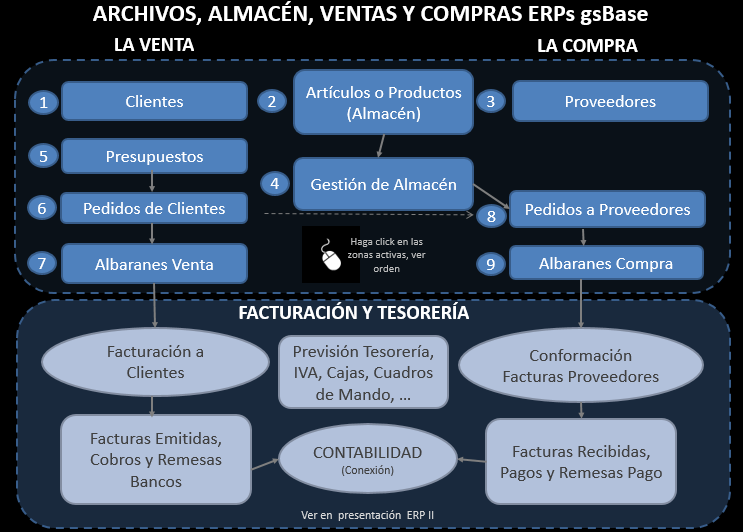
\includegraphics[scale=0.65]{imagenes/CapturasoftwareSaaS1a.png} 
	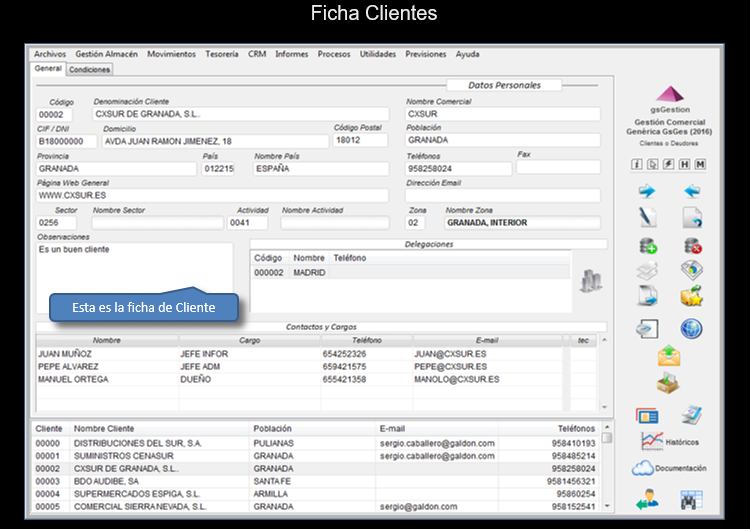
\includegraphics[scale=0.65]{imagenes/CapturasoftwareSaaS1b.png}
	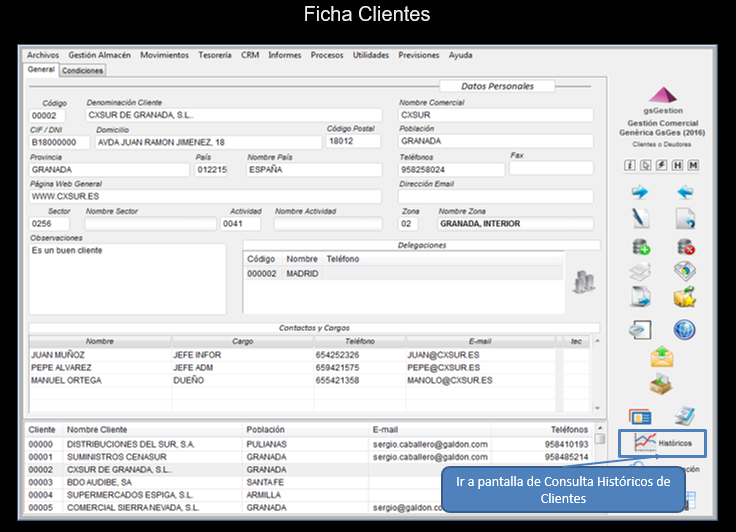
\includegraphics[scale=0.65]{imagenes/CapturasoftwareSaaS1c.png}
	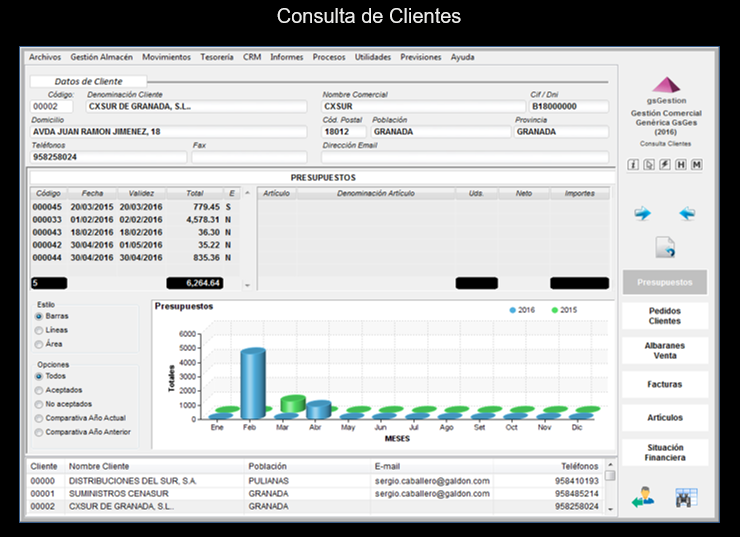
\includegraphics[scale=0.65]{imagenes/CapturasoftwareSaaS1d.png}
	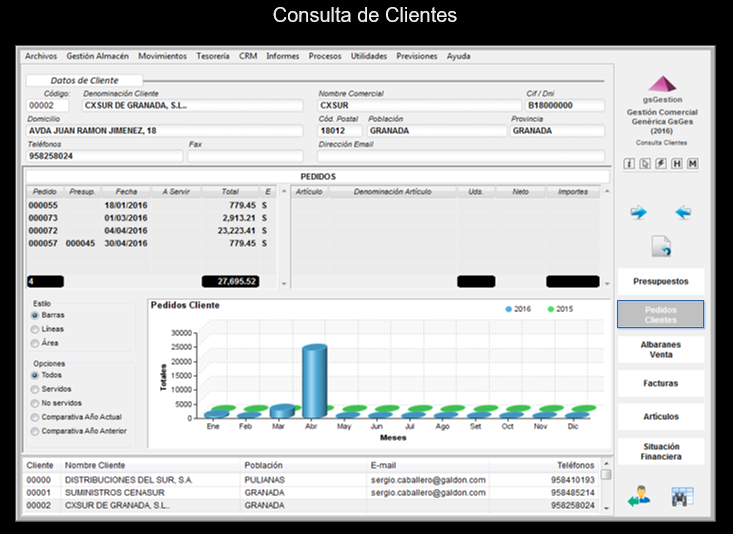
\includegraphics[scale=0.65]{imagenes/CapturasoftwareSaaS1e.png}
	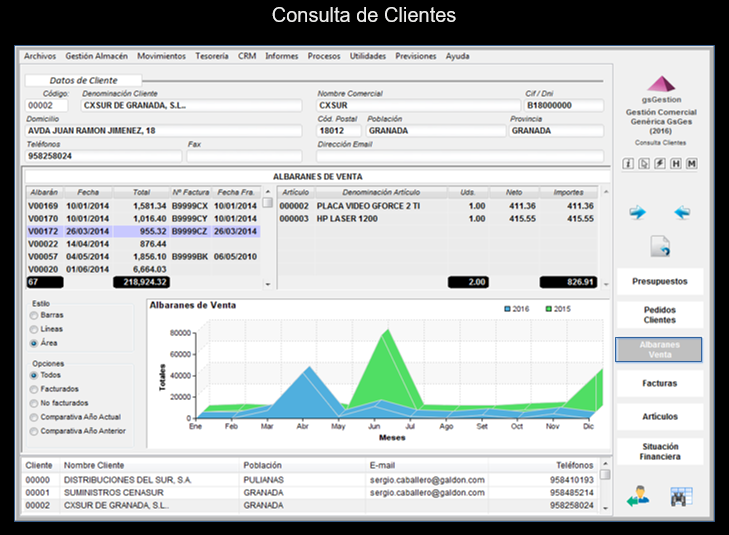
\includegraphics[scale=0.65]{imagenes/CapturasoftwareSaaS1f.png}
	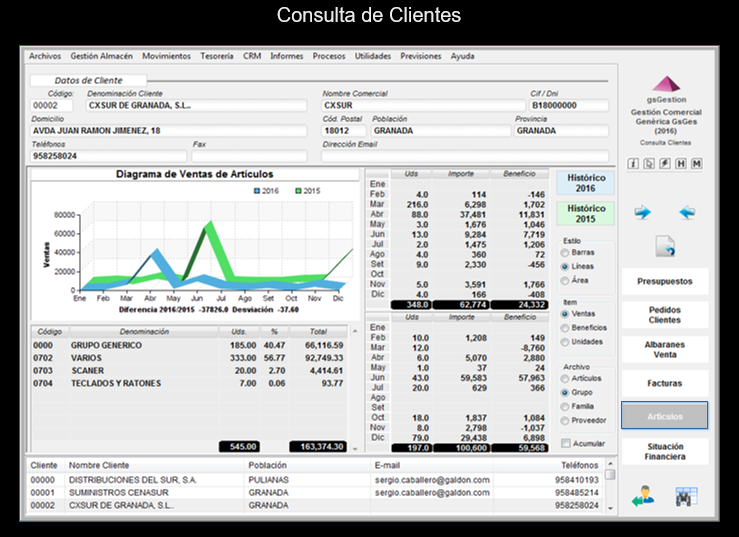
\includegraphics[scale=0.65]{imagenes/CapturasoftwareSaaS1g.png}
	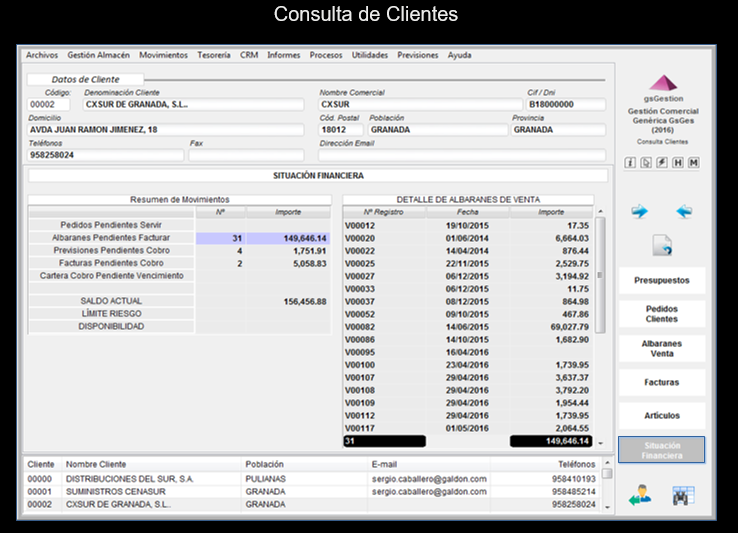
\includegraphics[scale=0.65]{imagenes/CapturasoftwareSaaS1h.png} 
	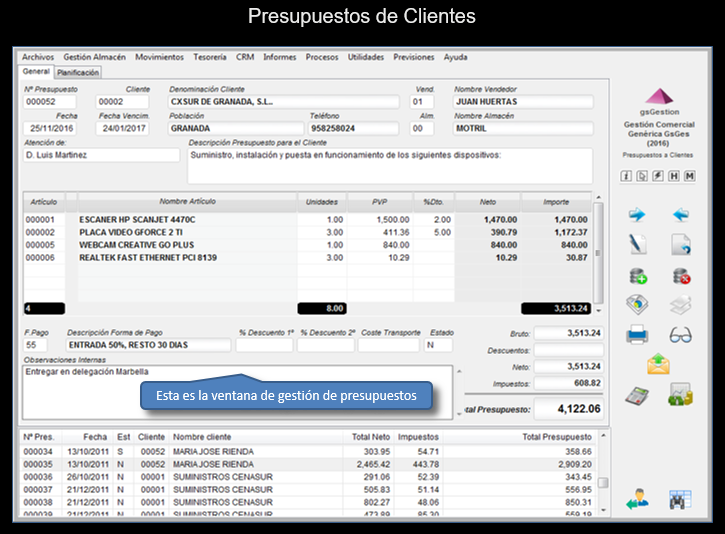
\includegraphics[scale=0.65]{imagenes/CapturasoftwareSaaS1i.png}
	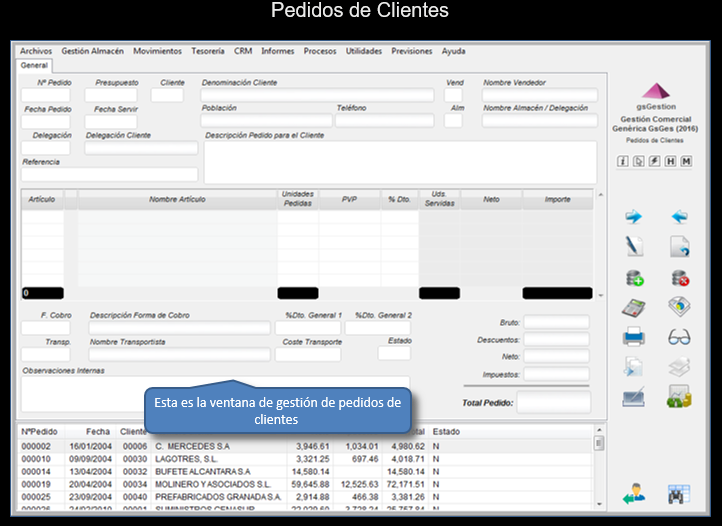
\includegraphics[scale=0.65]{imagenes/CapturasoftwareSaaS1j.png}
	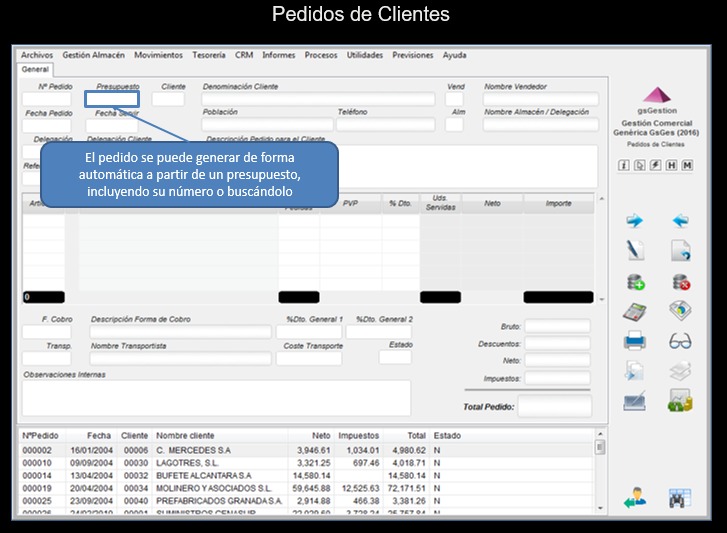
\includegraphics[scale=0.65]{imagenes/CapturasoftwareSaaS1k.png}
	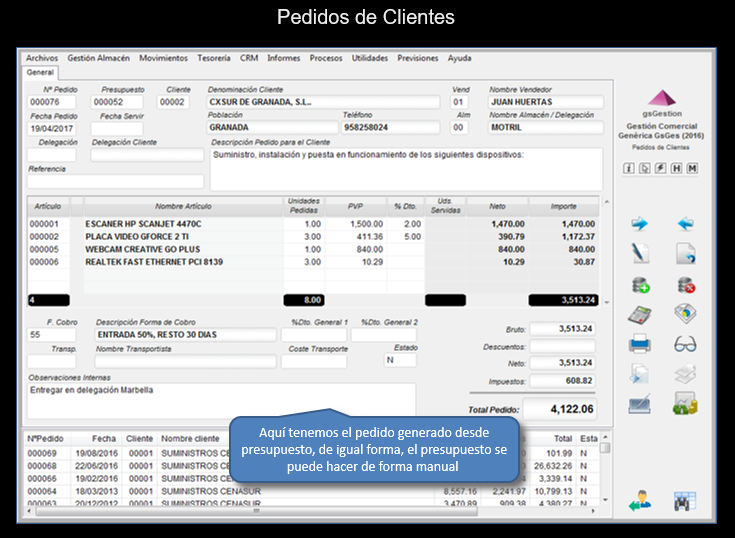
\includegraphics[scale=0.65]{imagenes/CapturasoftwareSaaS1l.png}
	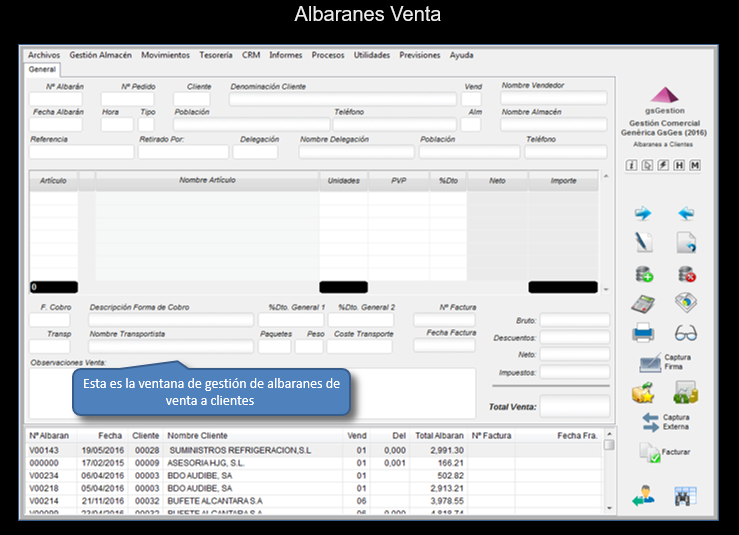
\includegraphics[scale=0.65]{imagenes/CapturasoftwareSaaS1m.png}
	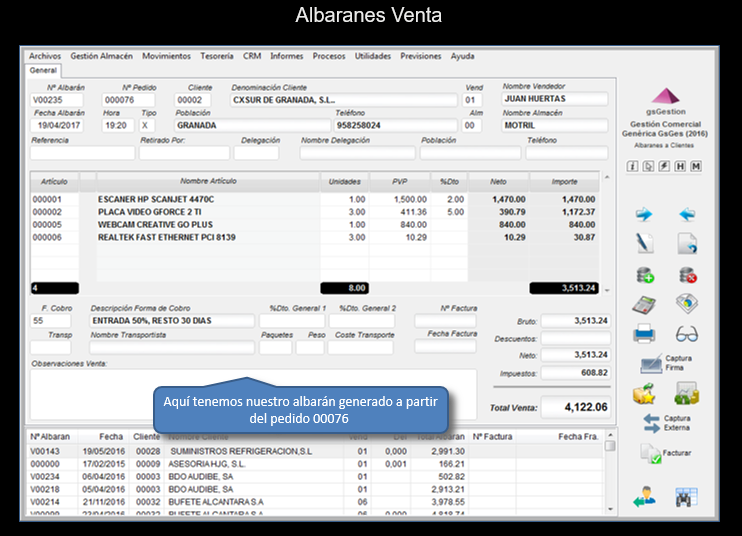
\includegraphics[scale=0.65]{imagenes/CapturasoftwareSaaS1n.png}
\end{flushleft}	

\end{itemize}
Todos sus softwares, aunque son totalmente personalizados, todos los ofertan y dan con vídeos de autoaprendizaje, lo que facilita y acomoda muchísimo más al cliente, mejorando la relación y atractivo por el producto que ofertan. 

Dan total comodidad a la hora de implantar cualquiera de sus productos, ya que se ofrecen a que sus propios técnicos sean los encargados de instalar el nuevo software y facilitarnos todo lo necesario para que el cliente tenga que realizar las menores acciones posibles. 

No obstante, al no tener unos cimientos fijos sobre los precios que pueden ofertar en función del servicio que queramos obtener hasta no contactar con ellos directamente, el cliente en una primera visión deberá de basar su credibilidad en sus casos de éxito, lo cual, dependiendo de cómo de buenos sean, les será beneficioso o no. 

\paragraph{Evaluación de Galdón:\\}

\begin{flushleft}
	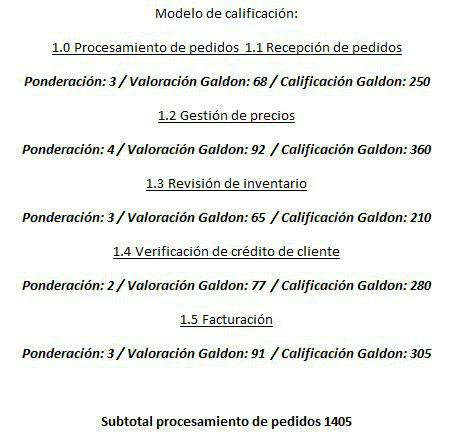
\includegraphics[scale=0.8]{imagenes/Galdon1.jpg}
	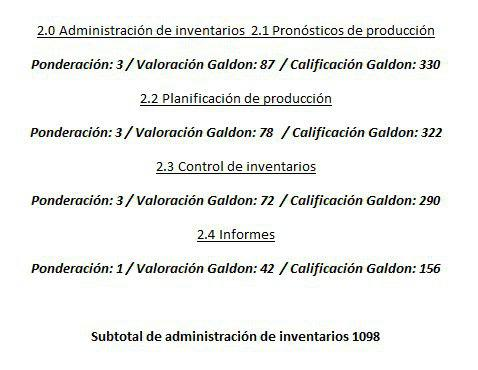
\includegraphics[scale=0.8]{imagenes/Galdon2.jpg}
	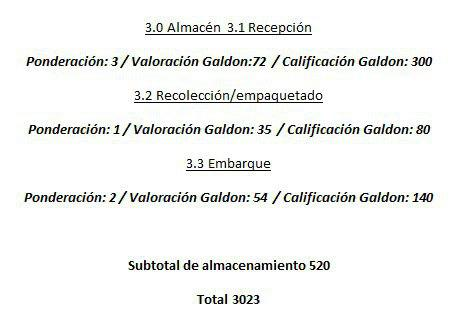
\includegraphics[scale=0.8]{imagenes/Galdon3.jpg}
\end{flushleft}

Criterios finalmente utilizados: Basándonos en el parcial desconocimiento del costo del producto final que pueda requerir un cliente, se valorará significativamente más el hecho de poder obtener un producto totalmente personalizado aunque la versión inicial requiera un coste grande ya que supondremos que la ganancia que aportará dicha inversión será equiparable a su precio, siendo éste, cuanto más elevado, mayor la ganancia (nunca sin llegar a los casos extremo) 

Escala usada para ponderar cada criterio: Suponiendo que pudiéramos pedir un software de gestión comercial como nosotros quisiéramos y viendo las prestaciones que ofrecen en cuanto a diseños personalizados, el software a primera vista no trata con problemas reales como el tamaño del producto a la hora de empaquetarlo ni qué caja sería la óptima, tanto en tamaño como en embalaje para el correcto transporte del producto (por eso la ponderación en el almacén es bastante baja). Sin embargo, al poder acceder a toda la información que necesitemos para administrar nuestro almacén, podremos tener una ponderación muy alta en éste secto

\subsection{Softwares de Movilidad}

\subsubsection{RepCamp}

	RepCamp es una plataforma cloud y móvil diseñada para mejorar las actividades comerciales de los representantes de ventas y optimizar al máximo el procesamiento de pedidos.  RepCamp se compone de una aplicación en la nube, una aplicación móvil y múltiples sistemas de sincronización. 

\begin{flushleft}
	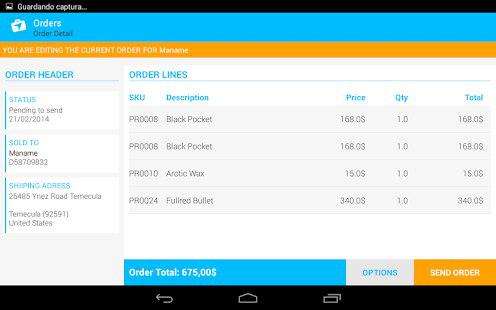
\includegraphics[scale=0.75]{imagenes/repcamp.jpg} 
\end{flushleft}

\paragraph{Criterios funcionales:}

\begin{itemize}

	\item \textbf{TPV (point of sale):} Un TPV multidivisa y con múltiples formas de pago, todas ellas configurables (efectivo, tarjetas, vales emitidos, vales de regalo, cheques, apertura de crédito, anticipos, etc.
	\item \textbf{Gestión del catálogo y precios:} Personalizable.
	\item \textbf{Gestión de devoluciones y cancelaciones:} Personalizable.
	\item \textbf{Facturación:} Personalizable.
	\item \textbf{Reserva de productos:} Personalizable.
	\item \textbf{Generación de informes:} Generación de documentos personalizada.
	\item \textbf{Soporte para métodos de pago:} El Punto de Venta proporciona un soporte para múltiples métodos de pago.

\end{itemize}

\paragraph{Criterios no funcionales:}

\begin{itemize}

	\item \textbf{Coste:} Desde 0 euros hasta 36 euros al mes.
	\item \textbf{Evolución:} Al incluir herramientas necesarias siempre, la evolución es positiva
	\item \textbf{Posibilidad de personalización:} Totalmente personalizable.
	\item \textbf{Casos de éxito:} COMPARFARM.

\end{itemize}

\paragraph{Evaluación de Recamp}

\begin{flushleft}
	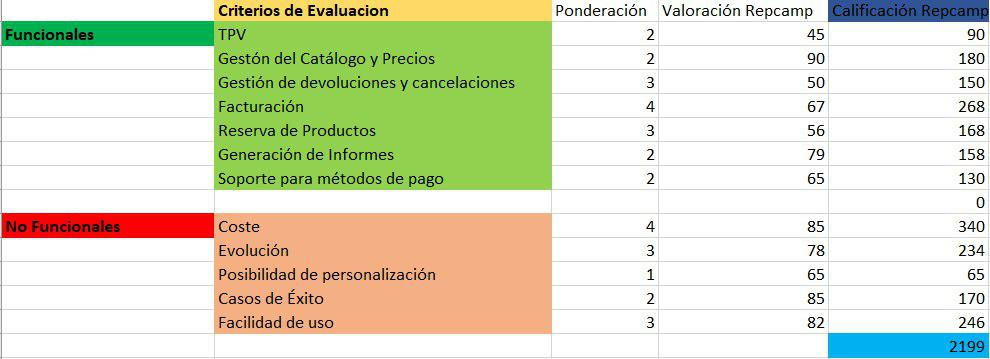
\includegraphics[scale=0.75]{imagenes/Repcamp.jpg} 
\end{flushleft}

\section{Conclusiones}



\begin{thebibliography}{9}

\bibitem{50Sage} \textit{50 Sage Cloud}, \url{https://www.sage.com/es-es/productos/sage-50-cloud/}.
\bibitem{CasosExito50Sage} \textit{Casos de éxito 50 Sage}, \url{http://partnews.sage.es/2018/01/caso-de-exito-sage-50c-con-office-365/}.
\bibitem{TPV50Sage} \textit{TPV 50 Sage}, \url{http://www.alcatic.com/sage-50-cloud/sage-50-cloud-tpv/}.
\bibitem{SaaSvsERP} \textit{Diferencias ERP tradicional y SaaS}, \url{https://www.gestionar-facil.com/software-de-gestion-erp-tradicional-vs-saas/}.
\bibitem{ERP} \textit{Definición ERP}, \url{https://www.galdon.com/erp-gestion-comercial-y-distribucion/}.
\bibitem{RepCamp} \textit{RepCamp}, \url{http://www.repcamp.com/es/index}.
\bibitem{RepCamp2} \textit{RepCamp}, \url{http://www.repcamp.com/es/plans}.
\bibitem{RepCamp3} \textit{RepCamp}, \url{http://www.repcamp.com/public/files/partners_es.pdf}.
\bibitem{TPVRepCamp} \textit{TPV en RepCamp}, \url{http://www.kriter.net/tecnologia-de-gestion-tpv}.
\bibitem{TPV2} \textit{Definición TPV}, \url{https://www.bbva.com/es/que-es-el-tpv/}.
\bibitem{CasosExitoRepCamp} \textit{Casos de éxito en RepCamp}, \url{http://www.kriter.net/images/files/PDF/Casos_exit/024_COMPARFARM.pdf}.
\bibitem{CasosExitoOdoo} \textit{Casos de éxito de Odoo}, \url{https://www.odoo.com/es_ES/page/cases}
\bibitem{FacturacionZFactura} \textit{Facturación ZFactura}, \url{https://www.ziclope.net/programas-de-facturacion/}
\bibitem{ZFactura} \textit{Videotutoriales ZFactura}, \url{https://www.ziclope.net/videotutoriales-zfactura/}
\bibitem{FacturaZFactura} \textit{Facturas ZFactura}, \url{https://www.modelofactura.net/programas/zfactura}
\bibitem{Gespymes} \textit{Gespymes}, \url{https://gespymes.es/}
\bibitem{DemoGespymes} \textit{Demos Gespymes}, \url{https://app.gespymes.es/licencias/demo_gespymes/index.php}

\end{thebibliography}



\end{document}